\chapter{Aircraft Longitudinal Static Stability}
\label{ch:workobject}
\markboth{Aircraft Longitudinal Static Stability}{}
\begin{flushright}
	{\smaller
		\textit{For every bad thing in life, \\ there are more good things to tip the balance.}\\
		--  Richelle Mead}
\end{flushright}


Static stability is the reaction of a body to a disturbance from equilibrium. To determine the static stability of a body, the body must be initially disturbed from its equilibrium state. If, when disturbed from equilibrium, the initial tendency of the body is to return to its original equilibrium position, the body displays positive static stability or is stable. If the initial tendency of the body is to remain in the disturbed position, the body is said to be neutrally stable. However, should the body, when disturbed, initially tend to continue to displace from equilibrium, the body has negative static stability or is unstable. \cite{airf}\\
In addition to the static stability it's possible to analize the dynamical stability that is the time history of an aircraft response after it has been disturbed, which is a more complete picture of aircraft behavior. A statically stable aircraft may not be dynamically stable, as explained in subsequent discussions. However, it is clear that a statically unstable aircraft also is dynamically unstable.

\begin{figure}[H]
\centering
{\includegraphics[height=8.3cm]{Immagini/stability}} 
\label{wblc}
\caption{Static and dynamic stability about the pitch axis.}
\end{figure} 		

It is important to note that there is a substantial difference between the concept of ``Stability'' and ``Equilibrium''. In fact, stability is a characteristic of an aircraft, while equilibrium is a state in which airplane can be, that means the equilibrium of the forces and the moments acting on it.\\
``Longitudinal static stability'' is the stability of an aircraft in the longitudinal, or pitching, plane under steady-flight conditions. This characteristic is important because an airplane must have the tendency to return to the equilibrium position if perturbed. The pitch plane is the XZ plane of aircraft symmetry. The linear velocities are along the X-axis and w along the Z-axis. Angular velocity is about the Y-axis , known as pitching (positive if nose up). Pilot-induced activation of the elevator changes the aircraft pitch. In the plane of symmetry, the aircraft motion is uncoupled; that is, motion is limited only to the pitch plane.\cite{kundu}\\

% aggiungi
 


% Per determinare stabilita longitudinale--> momento pitching rispetto al baricentro nullo. Quindi occorre calcolare tuutte le forze e i momenti dei vari componenti e poi calcolare il momento del aircraf. e chiaro che quest dipende dalla posizione del baricento.
%The forces and moments acting on an aircraft are shown in Fig. 21.4.
%The lift and drag are by defi nition always perpendicular and parallel to V∞,
%respectively. It is, therefore, inconvenient to use these forces to obtain
%moments because their moment arms relative to the center of gravity vary
%with angle-of-attack a. For this reason, all forces are resolved into normal,
%N, and chordwise, C, forces whose axes remain fi xed with the aircraft and
%whose arms are, therefore, constant:
%p589 nicolai


% scopo del piano di coda--> garantire equilibrio a diversi angoli.. sforza

% introduzione... stabilità, grafici e quali sono tutti i dati che servono
%Nicolai 585 
%Sforza 250
%kundu 387
%disegno stabilità
\section{Aerodynamic Lift}		
 Considering a reference angle of attack $\alpha_B$, the aircraft components generates lift. So it is necessary to evaluate these contributes. In particular, first of all, is wanted to evaluate the $C_L$ of isolated wing. This value will be correct with fuselage influence. Afterwards it is necessary to evaluate the contribute of horizontal tail.  It is important to note that each component works at a different angle of attack in dipendence of angles of incidence and downwash , meanwhile for longitudinal stability the reference angle of attack is $\alpha_B$.

\subsection{Wing}
\subsection{Fuselage}


The lift distribution on a wing is affected by the presence of the fuselage as a result of the following effects:
\begin{itemize}
\item The presence of the fuselage disturbs the longitudinal velocity field near the wing.
\item At an angle of attack relative to the free stream, the fuselage also perturbs the flow about the wing in planes normal to the free stream.
\item The fuselage has a blocking effect on the flow.
\end{itemize}
These effects are not large for a slender fuselage but may be important when the fuselage is relatively bulky, so that a substantial alteration to the local longitudinal velocity may result. The cross-flow caused by the fuselage at angle of attack changes the component of free stream velocity normal to the fuselage axis and affects the downwash flow produced by the wing. \cite{sforza2014commercial}
However, theoretical analysis showed that the presence of a slender fuselage does not have an important effect on the lift
distribution on an unswept wing of moderate aspect ratio, but a larger change in the lift distribution on a wing in the presence of a fuselage may be anticipated if the wing is swept.\cite{zlotnick}
For greater accuracy of the calculation, the value of lift linear slope has been corrected using the following equation from \cite{roskammethods}:

\begin{equation}
\left ( \frac{d C_L}{d\alpha} \right)_{w \!b} = \left[ 1 + \frac{1}{4} \left ( \frac {d}{b} \right ) - \frac{1}{40} \left (\frac{d}{b} \right) ^2 \right] \left ( \frac{d C_L}{d\alpha} \right)_{w}
\end{equation}

Note that for typical airliners $\frac{d}{b} \approx 0.1$ and therefore the lift curve slope of the wing-body is approximately equal to that of the wing alone.\\
In addition to the calculation of the linear slope of the wing body group, it is necessary to calculate the intersection point between the lift curve of wing and the lift curve of wing-body. This point is the $\alpha_{0_L}$ of the exposed wing, that is the wing outside the fuselage. This value has been calculated with the integral formula.

\begin{equation}
\alpha_{0L} |_{EW} = \frac{2}{S_E}\int_{y_{0_E}}^{\frac{b}{2}} c(y) [ \alpha_0(y_E) - \epsilon_T(y_E) ] \, dy
\end{equation}


\begin{figure}[H]
\centering
{\includegraphics[height=8.4cm]{Immagini/WingBody_CL_Vs_alpha_curve}} 
\label{wblc}
\caption{Lift curve of isolated wing and of wing-body group.}
\end{figure} 		


\subsection{Horizontal Tail}
The H-tail consists of the stabilizer (fixed or moving) and the elevator (moving) for handling the pitch degree of freedom. The H-tail can be positioned low through the fuselage, in the middle cutting through the V-tail, or at the top of the V-tail to form a T-tail. \cite{kundu}
%nicolai p 283
\subsubsection{Elevator index of effectiveness}
 In order to evaluate the contribution to the longitudinal stability of horizontal tail it's necessary to consider the deflection of the elevator. 
		
\begin{figure}[H]
\centering
{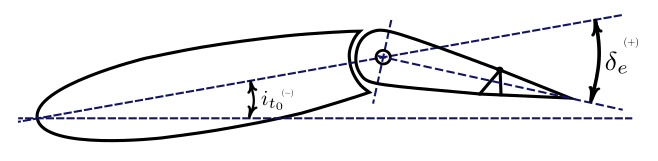
\includegraphics[height=2.3cm]{Immagini/horizontal_tail_profile_deltaE.pdf}} 
\label{htailangle}
\caption{Characteristic angles of the horizontal tail.}
\end{figure} 		
		
The variation of zero lift angle is not constant with the angle of deflection. So it's necessary to evaluate the tau factor which is defined as follows:

\begin{equation}		 
\tau_e = \frac{d \alpha_{0l}}{d \delta_e}
\end{equation}

		
Introducing this parameter the lift coefficient of the horizontal tail can be rated as follows:

\begin{equation}
C_{L_H}= C_{L_0} + C_{L_{{\alpha}_H}} \alpha_H + 	C_{L_{{\alpha}_H}} \tau_e \delta_e
\end{equation}

  
Considering a symmetrical horizontal tail, the term $C_{L_0}$ is zero, so it's possible to express the lift coefficient in the following form:


\begin{equation}
C_{L_H}= C_{L_{{\alpha}_H}} \left ( \alpha_H + \tau_e \delta_e \right)
\end{equation}
  		
 In general the value of $\tau$ is constant until about 15 deg; after this value, due to the flow separation, the effectiveness of elevator decrease and consequently the product $ \tau_e \delta_e$ that appears in the equation of lift coefficient.
		
%grafici di progetto.


\begin{figure}[H]
\centering
{\includegraphics[height=6.79cm]{Immagini/taude.png}} 
\label{tau1}
\caption{Qualitative trend of $\tau$ with the deflection of elevator.}
\end{figure} 		


\begin{figure}[H]
\centering
{\includegraphics[height=6.79cm]{Immagini/taudeltae.png}} 
\label{tau2}
\caption{Qualitative trend of the term $\tau \cdot \delta_e$ with the deflection of elevator.}
\end{figure} 		


\begin{figure}[H]
\centering
{\includegraphics[height=4.9cm]{Immagini/tau.png}} 
\label{tau3}
\end{figure} 		


		
The evaluation of tau is made by reading of external database, considering the following graphs.
	
\begin{equation}
\tau = \alpha_{\delta} \eta_{\delta} = \frac{\alpha_{{\delta}_{c_L}}}{\alpha_{{\delta}_{c_l}}}\alpha_{{\delta}_{c_l}} \eta_{\delta}
\end{equation}



%\begin{figure}[H]
%\centering
%{\includegraphics[height=6cm]{Immagini/Eta_Delta_Plain.png}} 
%\caption{2D efficiency correction for elevator.}
%\label{efficiency}
%\end{figure} 		
%
%
%\begin{figure}[H]
%\centering
%{\includegraphics[height=6cm]{Immagini/alfadelta.png}} 
%\caption{$\frac{d \alpha_{0l}}{d \delta_e}$ 2D and 3D correction.}
%\label{efficiency}
%\end{figure} 		

\begin{figure}[H]
\centering
{\includegraphics[height=6.79cm]{Immagini/alfadeltanew.png}} 
\label{efficiency}
\end{figure} 		


		
% java class archiecture(?)
%tabella elenco metodi con classe e che fanno

% descrizione

% spiegazione  (da fare) del calcolo del cl at alfa simile a quello dell ala
% spiegazione (da fare )  metodo calcolo tau in stability calculator
% spiegazione (gia fatta) del metodo calculateclwithdeflection in ls aerodynamic

% grafici con risultati

\subsection{Complete Aircraft}

In order to evaluate the lift coefficient of the entire airplane it's possible to consider it as consisting of the following parts\cite{ roskam2002airplane}:

\begin{itemize}
\item Wing and Fuselage
\item Horizontal Tail
\item Canard
\end{itemize}

It's important to consider the effectiveness angles of attack in which the surfaces work. This is made considering the angles of incidence of the lifting surfaces and the downwash angle aft of the wing. An horizontal tail and a canard may be equipped with a trailing edge control surface. So in order to evaluate these contributes it's important to know the angle of deflection $\delta$ of these control surfaces.\\
The calculation of the individual contributions it's reported in the relevant sections. In this section will be shown the method to evaluate the aircraft lift coefficient, known the single contributes.\\
For an aircraft with no canard, the formula is the following:

\begin{equation}
C_L = C_{L_{wb}} + \frac{S_t}{S_w} \eta_t C_{L_{t}}
\end{equation}

Where $\eta_t$ is the ratio of dynamic pressure. In fact the dynamic pressure seen by horizontal tail differ from the free stream dynamic pressure due to two main reasons: the combination wing-fuselage and the presence of the propeller. The dynamic pressure of the tail depends on the location of the tail. If the tail is in the wake of the wing-body, the local dynamic pressure will be less than the freestream because the flow gradually loses its kinetic energy. While if the tail is in the slipstream of propeller, the local dynamic pressure may increase due to the power absorbed by the propeller.



\section{Aerodynamic Drag}
% nell' ottica di questo lavoro divideremo per componente
% foto divisione p 387 sforza pdf
% mettiamo ala piano coda e fusoliera
\subsection{Wing}
\subsection{Fuselage}
\subsection{Horizontal Tail}
% contributo dovuto al flap


\section{Pitching Moments}
\subsection{Wing}
\subsection{Fuselage}
\subsection{Horizontal Tail}
\subsection{Propulsors}

\subsection{Stability Calculation}

% calcolo delle forze normali e tangenziali, calcolo momenti, risultati

\section{Java Class Architecture}
% intro
% riepilogo di tutte le classi in schema. vedi su quaderno  prima di stabilita
% schema in yed

\section{User's Guide}
%intro
% test class

\section{Analysis Results} % fai qui? oppure durante?
%grafici